\subsection{Interfaz de la sección ``Producciones''}
La interfaz de esta sección consiste principalmente en una tabla donde el administrador podrá ver la información de las producciones que se han creado. Las columnas que conforman esta tabla son: folio, lote, producto, piezas, fecha de creación, estatus, persona que generó la producción, persona que modificó la producción y las acciones que se pueden realizar; además, cada columna puede ser ordenada de manera ascendente o descendente al presionar su nombre, y también se puede seleccionar la columna para realizar una busqueda de información.

Del lado izquierdo de la tabla se encuentra un menú que contiene un botón que permite crear las producciones y una cuenta de las producciones que se encuentran en diferentes estatus (Ver Figura 38).

    \begin{figure}[H]
        \begin{center}
            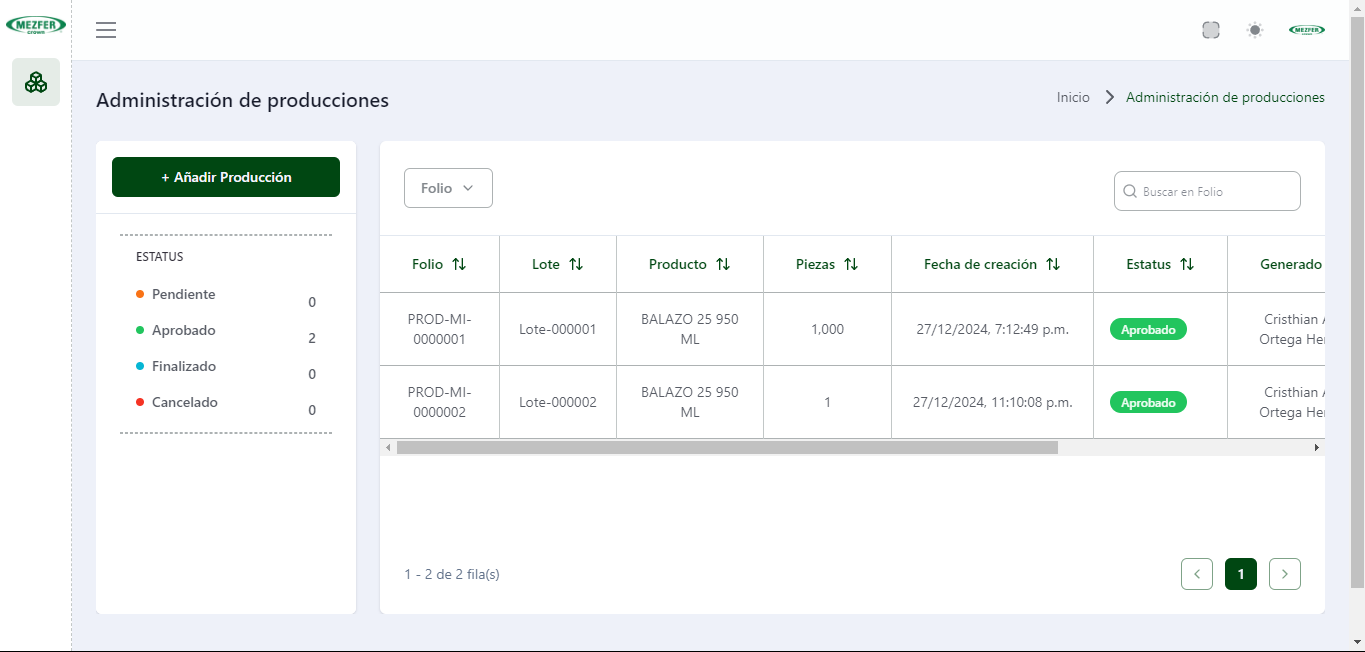
\includegraphics[scale=0.33]{img/actividades/producciones/interfaz-producciones.png}
            \caption{Interfaz principal de la sección de producciones.}
            \label{fig:interfaz-producciones}
        \end{center}
    \end{figure}

Cuando se presiona el botón que se encuentra en el menú lateral de la tabla, el que tiene la leyenda ``+ Añadir Producción'', se mostrará un Dialog que contiene un formulario con los campos necesarios para crear la producción. Estos campos son:
    \begin{itemize}
        \item Un componente llamado ``Select'' que muestra una lista de productos para seleccionar.
        \item Un campo donde se ingresa el lote de la producción.
        \item Un campo donde se ingresa la cantidad de piezas que se van a producir.
    \end{itemize}

El Dialog contiene un botón con la leyenda ``Crear'', que al presionarlo manda la información del formulario al Backend para procesarla y guardarla en la base de datos (Ver Figura 39).

    \begin{figure}[H]
        \begin{center}
            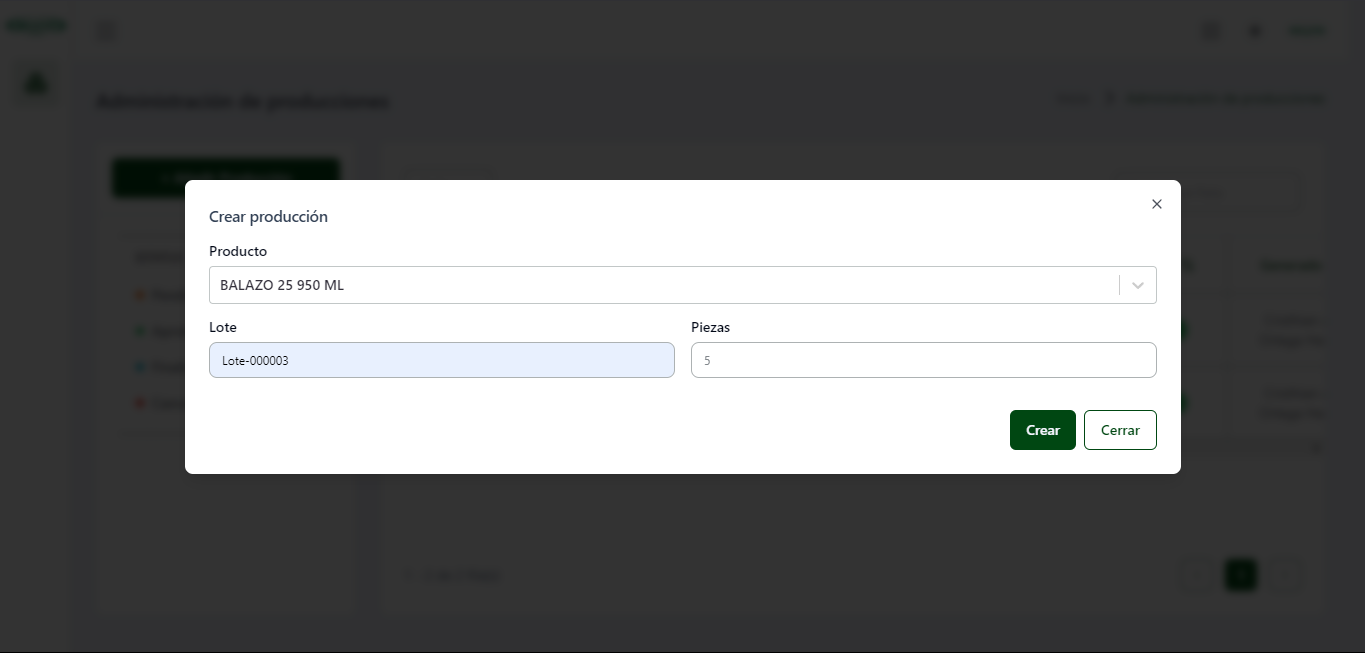
\includegraphics[scale=0.33]{img/actividades/producciones/formulario-producciones.png}
            \caption{Formulario para crear producciones.}
            \label{fig:formulario-producciones}
        \end{center}
    \end{figure}

La nueva producción creada se mostrará en la tabla y tendrá el estatus ``Pendiente'' por defecto. Cuando una producción tiene este estatus, en la columna ``Acciones'' de la tabla aparecerán 3 botones que permiten realizar diferentes acciones (Ver Figura 40). 

    \begin{figure}[H]
        \begin{center}
            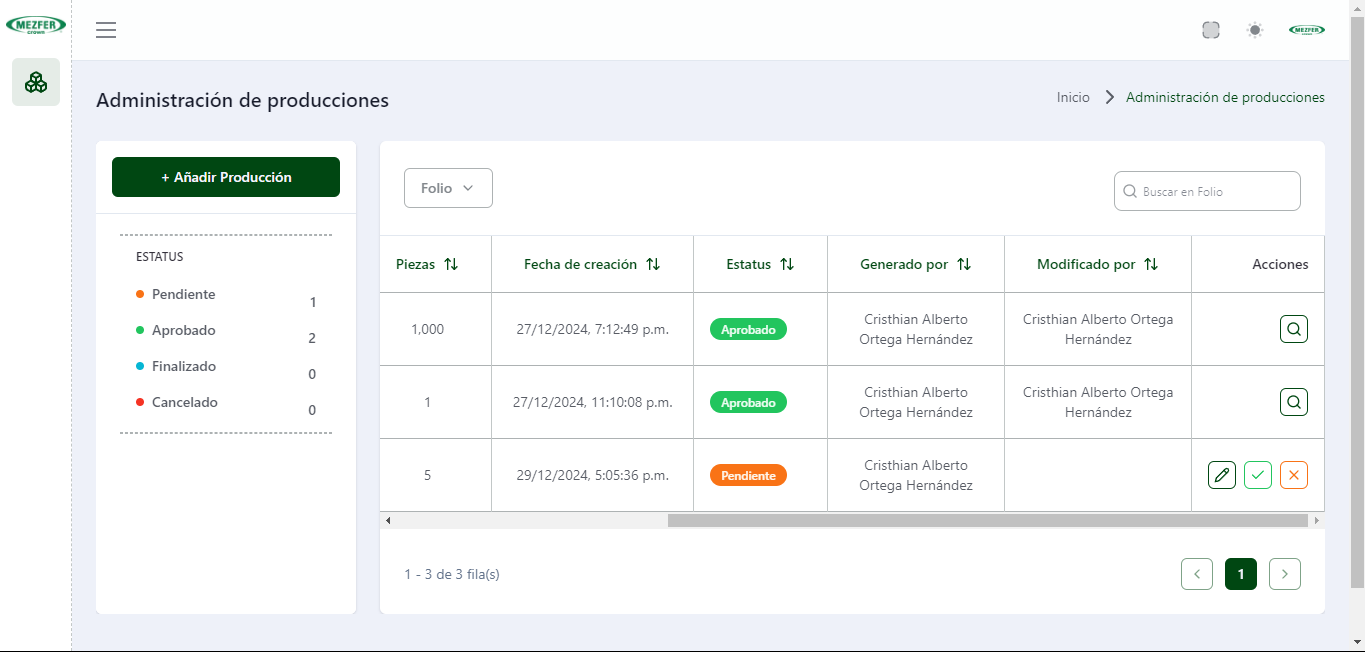
\includegraphics[scale=0.33]{img/actividades/producciones/botones-accion.png}
            \caption{Botones de acción en las nuevas producciones.}
            \label{fig:botones-accion}
        \end{center}
    \end{figure}

Como se mencionó anteriormente, cada uno de estos botones realiza algo diferente, por lo que se explicará la funcionalidad de cada uno de ellos.

El botón verde que tiene el ícono de un lapiz es el que permite al administrador cambiar la información de la producción. Al presionarlo, se mostrará un Dialog con el mismo formulario que se muestra al crear una nueva producción, la diferencia está en que ahora los campos ya vendrán completados con la información existente. El formulario detecta si se han realizado cambios en la información; si no se ha realizado ningún cambio, el botón de confirmación queda deshabilitado para evitar una petición innecesaria al backend, pero si se ha realizado algún cambio, el botón se habilita y en el cuerpo de la solicitud sólo se manda el campo que ha sido modificado (Ver Figura 41).

    \begin{figure}[H]
        \begin{center}
            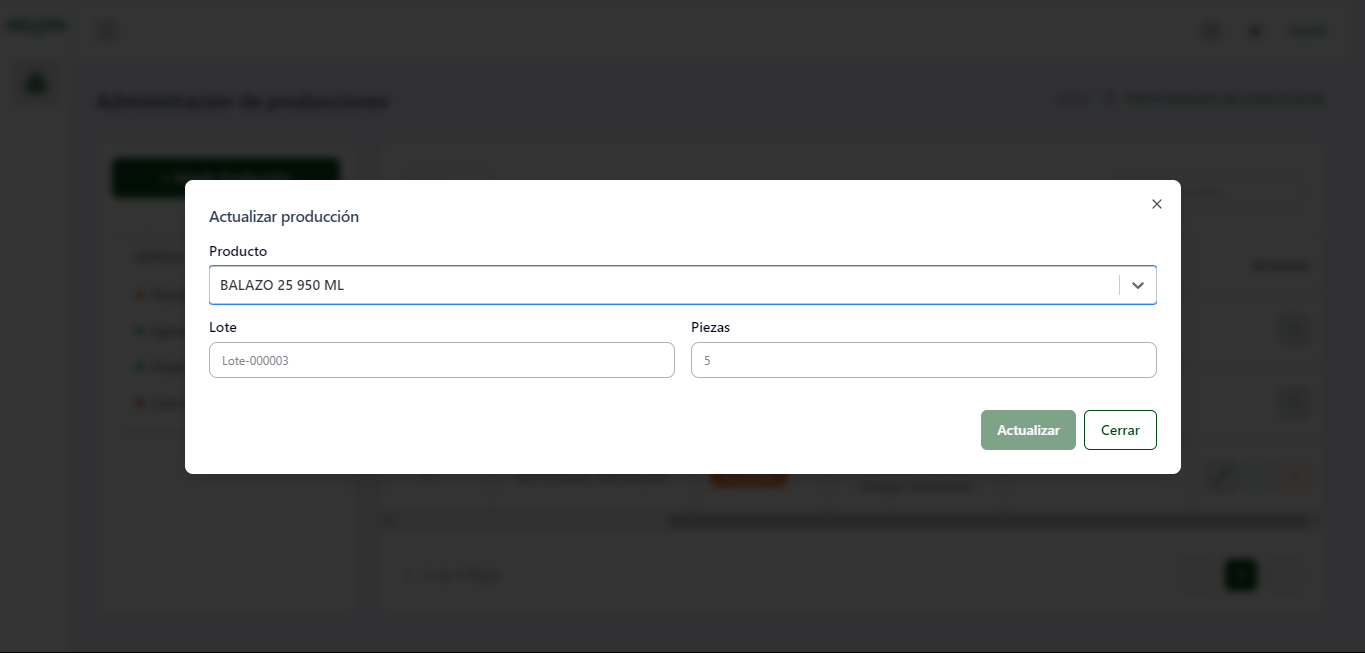
\includegraphics[scale=0.33]{img/actividades/producciones/formulario-update.png}
            \caption{Formulario para actualizar información de producciones.}
            \label{fig:formulario-update}
        \end{center}
    \end{figure}

El botón naranja que tiene el ícono de una equis es el que permite cambiar el estatus de la producción a ``Cancelado''. Al presionarlo se mostrará un Dialog con una advertencia indicando que está por cambiar el estatus de la producción y que, al cambiarlo, ya no se podrán realizar cambios en la información y se deberá confirmar o cerrar la advertencia (Ver Figura 41).

    \begin{figure}[H]
        \begin{center}
            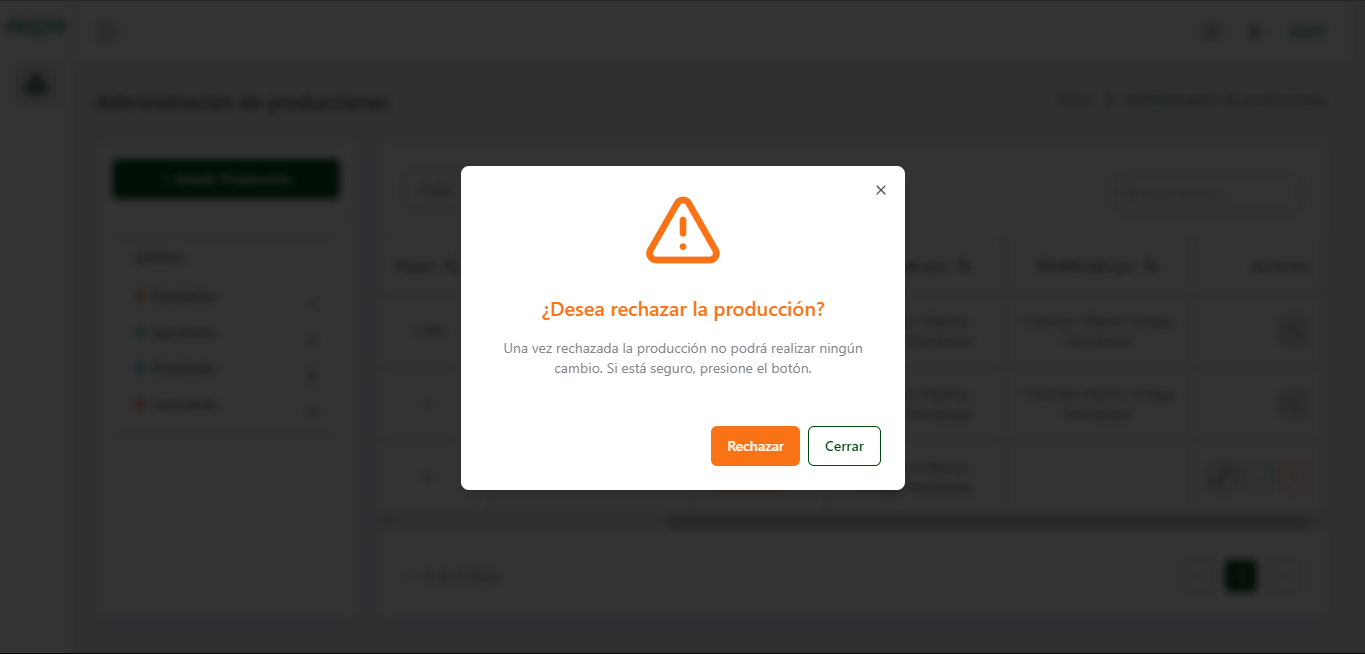
\includegraphics[scale=0.33]{img/actividades/producciones/advertencia-cancelada.png}
            \caption{Advertencia para cancelar una producción.}
            \label{fig:advertencia-cancelada}
        \end{center}
    \end{figure}

Una vez cancelada la producción, ya no se podrán realizar más acciones, por lo que la columna de ``Acciones'' quedará vacía para cada una de las producciones que tengan este estatus.

El otro botón verde que tiene el ícono de una tic es el que permite cambiar el estatus de la producción a ``Aprobado''. Al presionarlo ocurrirá lo mismo que con el botón anterior, se mostrará una advertencia y se tendrá que realizar una confirmación o cerrar la advertencia.

    \begin{figure}[H]
        \begin{center}
            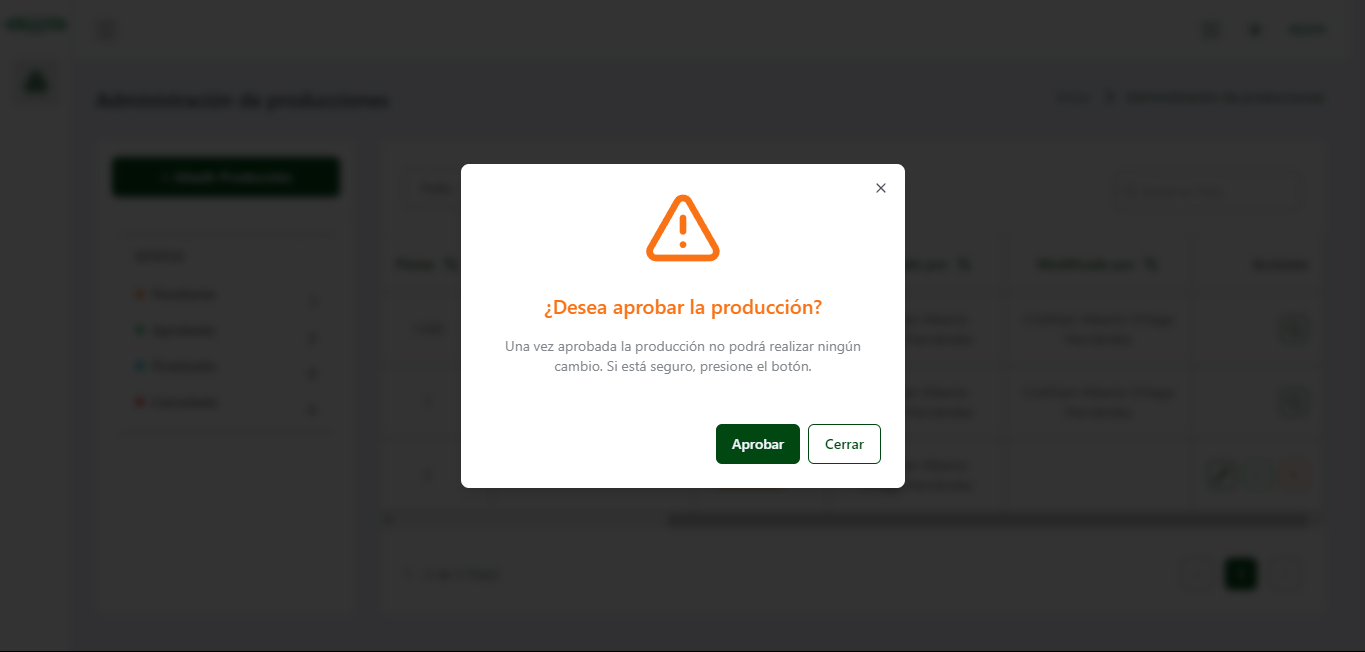
\includegraphics[scale=0.33]{img/actividades/producciones/advertencia-aprobado.png}
            \caption{Advertencia para aprobar una producción.}
            \label{fig:advertencia-aprobado}
        \end{center}
    \end{figure}

Si se confirma el cambio de estatus, la cantidad de piezas que hayan sido indicadas en la producción se crearán y los botones que se encontraban en la columna de ``Acciones'' cambiarán, ahora se mostrará un botón con el ícono de una lupa. Al presionar este botón se mostrará un Dialog con una tabla, y esta tabla contiene los detalles de la producción, es decir, las piezas que se crearon (Ver Figura 44).

    \begin{figure}[H]
        \begin{center}
            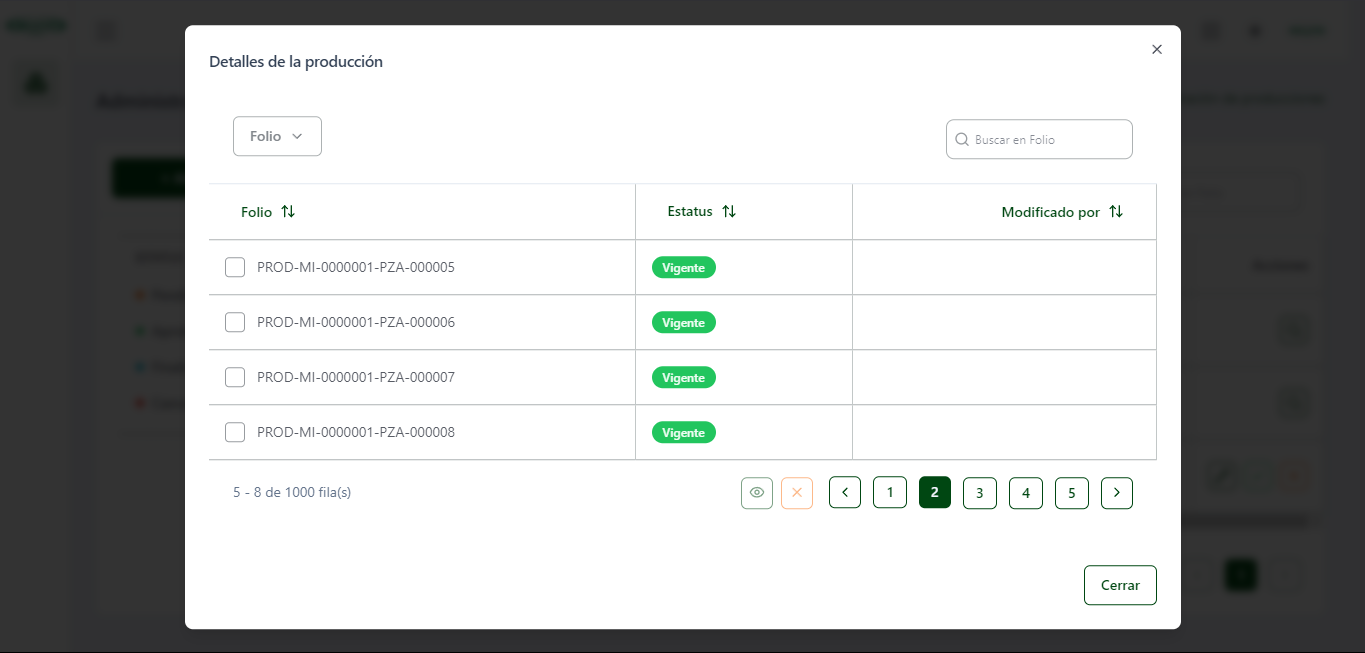
\includegraphics[scale=0.33]{img/actividades/producciones/prod-detalles.png}
            \caption{Dialog con los detalles de la producción.}
            \label{fig:prod-detalles}
        \end{center}
    \end{figure}

Esta tabla tiene la característica de que permite realizar acciones en lote, es decir, que una misma acción se realice para un conjunto de registros. Del lado izquierdo de cada registro se encuentra un Checkbox que permite seleccionar los registros a los que se les va a aplicar una acción; mientras no haya registros seleccionados, los botones que se encuentran en la parte inferior de la tabla permanecerán deshabilitados.

Al igual que en la tabla principal, esos botones sirven para cambiar el estatus de los registros. El botón verde que tiene el ícono de un ojo permite cambiar el estatus del registro a ``Leído'' mientras que el btoón naranja que tiene el ícono de una equis cambia el estatus a ``Cancelado''. Al presionar cualquiera de los botones se mostrará un Dialog con una advertencia indicando que se cambiará el estatus del registro y que la acción no se podrá deshacer (Ver Figuras 45 y 46).

    \begin{figure}[H]
        \begin{center}
            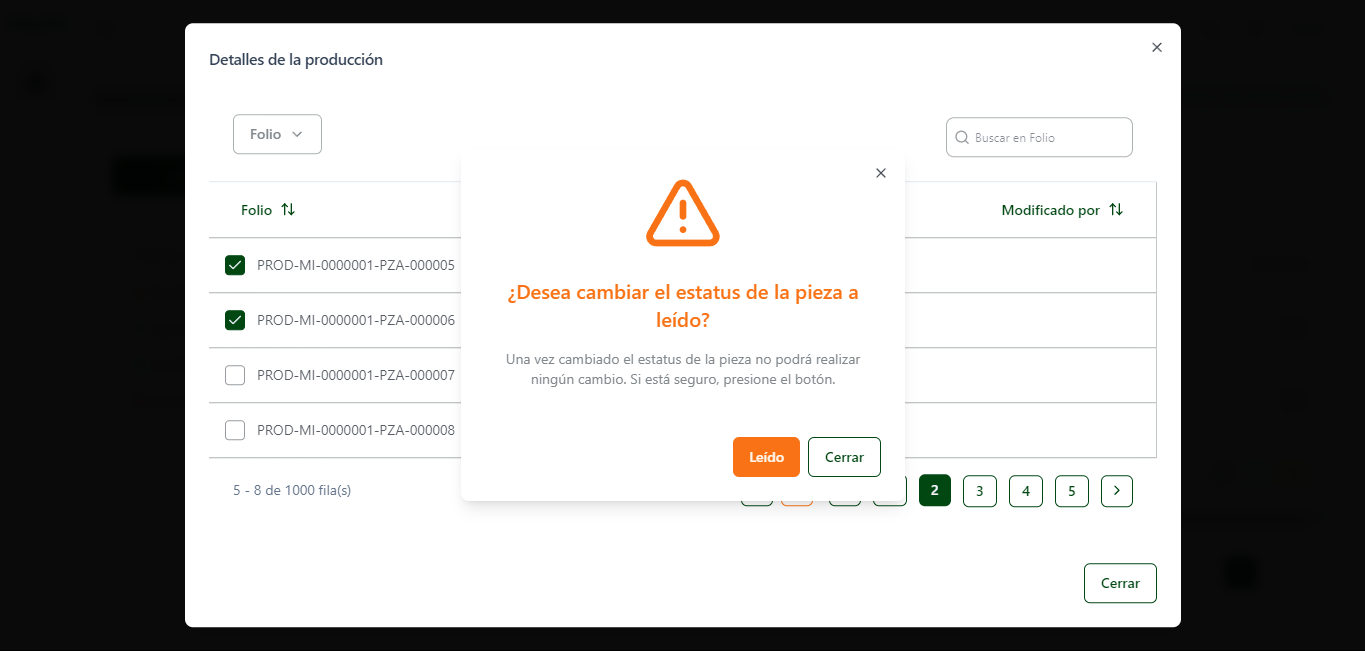
\includegraphics[scale=0.33]{img/actividades/producciones/registro-leido.png}
            \caption{Advertencia para cambiar el estatus a leído de un registro.}
            \label{fig:registro-leido}
        \end{center}
    \end{figure}

    \begin{figure}[H]
        \begin{center}
            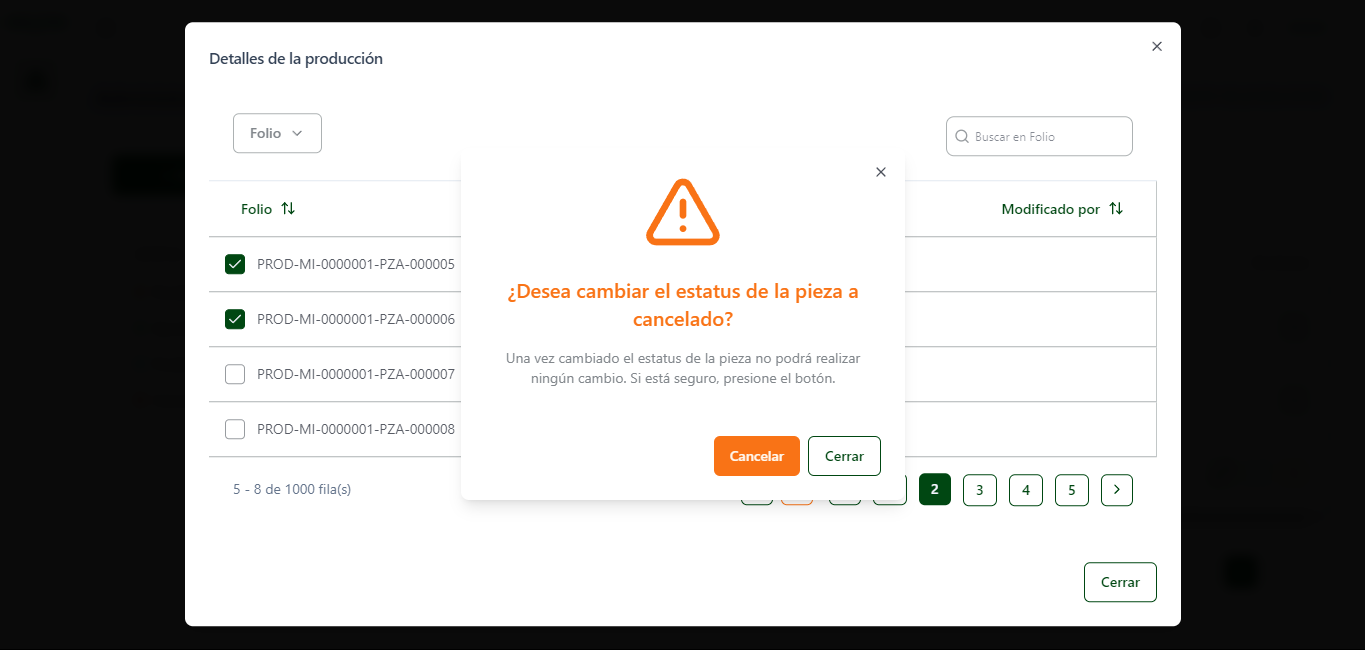
\includegraphics[scale=0.33]{img/actividades/producciones/registro-cancelado.png}
            \caption{Advertencia para cambiar el estatus a cancelado de un registro.}
            \label{fig:registro-cancelado}
        \end{center}
    \end{figure}

Como último detalle a mencionar, tanto en la tabla principal como en la tabla de los detalles existe una columna llamada ``Modificado por'' en la cual se muestra el nombre de la persona que realizó alguna modificación en la producción o en las piezas. Cuando son nuevos registros, esta columna siempre inicia vacía pues no ha habido alguien que les haya hecho un cambio, pero cuando se les cambia el estatus, esta columna se actualiza con el nombre de la persona que realizó el cambio. 